\documentclass[12pt,a4paper]{article}
\usepackage[utf8]{inputenc}
\usepackage[T1]{fontenc}
\usepackage[croatian]{babel}
\usepackage{geometry}
\usepackage{graphicx}
\usepackage{setspace}
\usepackage{titlesec}
\usepackage{fancyhdr}
\usepackage{caption}
\usepackage{tabularx}
\usepackage{amsmath}
\usepackage{tikz}
\usepackage{pgfplots}
\pgfplotsset{compat=1.18}

\geometry{left=3cm,right=2.5cm,top=2.5cm,bottom=2.5cm}
\onehalfspacing

\titleformat{\section}{\normalfont\Large\bfseries\uppercase}{\thesection.}{1em}{}
\titleformat{\subsection}{\normalfont\large\bfseries}{\thesubsection.}{1em}{}
\titleformat{\subsubsection}{\normalfont\normalsize\bfseries}{\thesubsubsection.}{1em}{}

\renewcommand{\contentsname}{SADRŽAJ}
\renewcommand{\listfigurename}{POPIS SLIKA}
\renewcommand{\listtablename}{POPIS TABLICA}

\begin{document}

\begin{titlepage}
    \centering
    {\large SVEUČILIŠTE U ZAGREBU\\}
    {\large FAKULTET STROJARSTVA I BRODOGRADNJE\\}
    \vspace{2.5cm}
    {\Large DIPLOMSKI RAD\\}
    \vspace{1.5cm}
    {\Huge \textbf{RAZVOJ I IMPLEMENTACIJA AUTONOMNOG SUSTAVA}\\}
    \vspace{1.5cm}
    {\large Ivan Horvat\\}
    \vfill
    {\large Zagreb, 2026.}
\end{titlepage}

\begin{titlepage}
    \thispagestyle{empty}
    \centering
    {\large SVEUČILIŠTE U ZAGREBU\\}
    {\large FAKULTET STROJARSTVA I BRODOGRADNJE\\}
    \vspace{2.5cm}
    {\Large DIPLOMSKI RAD\\}
    \vspace{1.25cm}
    {\Large \textbf{RAZVOJ I IMPLEMENTACIJA AUTONOMNOG SUSTAVA}\\}
    \vspace{1.5cm}
    
    \begin{minipage}[t]{0.45\textwidth}
        \begin{flushleft}
            \large Mentori:\\
            prof. dr. sc. Pero Perić
        \end{flushleft}
    \end{minipage}
    \hfill
    \begin{minipage}[t]{0.45\textwidth}
        \begin{flushright}
            \large Student:\\
            Ivan Horvat
        \end{flushright}
    \end{minipage}

    \vfill
    \begin{minipage}{0.9\textwidth}
    \noindent Izjavljujem da sam ovaj rad izradio samostalno koristeći znanja stečena tijekom studija i navedenu literaturu.
    \end{minipage}

    \vspace{1.5cm}

    \begin{minipage}{0.9\textwidth}
    \noindent Zahvaljujem se svima.
    \end{minipage}

    \vspace{2cm}
    {\large Ivan Horvat}
\end{titlepage}

\pagenumbering{roman}
\tableofcontents
\newpage
\listoffigures
\newpage
\listoftables
\newpage
\pagenumbering{arabic}

\section{1. UVOD}
Ovo je uvodni dio diplomskog rada. Sustav se razvija u svrhu optimizacije industrijskih procesa. U radu se analiziraju suvremene metode upravljanja i umjetne inteligencije primjenjive u robotici.

\section{2. METODOLOGIJA I RAZRADA}
Ovo poglavlje detaljno opisuje implementaciju.

\subsection{2.1. Arhitektura sustava}
Arhitektura se temelji na modularnom pristupu. Komunikacija između modula ostvaruje se putem brze lokalne mreže.

\subsection{2.2. Algoritmi upravljanja}
Upravljački algoritmi implementirani su korištenjem Pythona.

\subsubsection{2.2.1. PID regulator}
PID regulator osigurava stabilnost sustava u zatvorenoj petlji.

\subsubsection{2.2.2. RAG sustav umjetne inteligencije}
Sustav koristi Retrieval-Augmented Generation za donošenje odluka.

Slika \ref{fig:dummy} prikazuje pojednostavljeni model.
\begin{figure}[h]
    \centering
    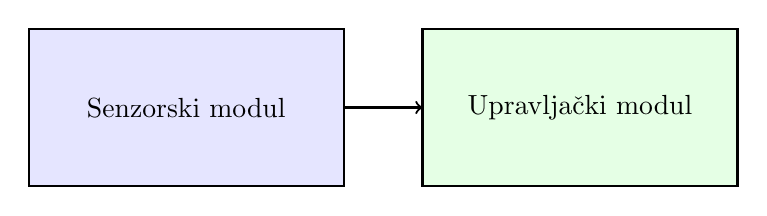
\begin{tikzpicture}
        \draw[thick, fill=blue!10] (0,0) rectangle (4,2);
        \node at (2,1) {Senzorski modul};
        \draw[thick, fill=green!10] (5,0) rectangle (9,2);
        \node at (7,1) {Upravljački modul};
        \draw[thick, ->] (4,1) -- (5,1);
    \end{tikzpicture}
    \caption{Blok shema sustava}
    \label{fig:dummy}
\end{figure}

Tablica \ref{tab:rezultati} prikazuje izmjerene parametre.
\begin{table}[h]
    \centering
    \caption{Parametri PID regulatora}
    \label{tab:rezultati}
    \begin{tabularx}{0.8\textwidth}{|X|X|X|}
        \hline
        \textbf{Parametar} & \textbf{Vrijednost} & \textbf{Jedinica} \\ \hline
        $K_p$ & 1.5 & - \\ \hline
        $K_i$ & 0.1 & $s^{-1}$ \\ \hline
        $K_d$ & 0.05 & $s$ \\ \hline
    \end{tabularx}
\end{table}

\subsection{2.3. Simulacijski model}
U nastavku je prikazan graf odziva sustava na jedinični skok (Slika \ref{fig:graf}).

\begin{figure}[h]
    \centering
    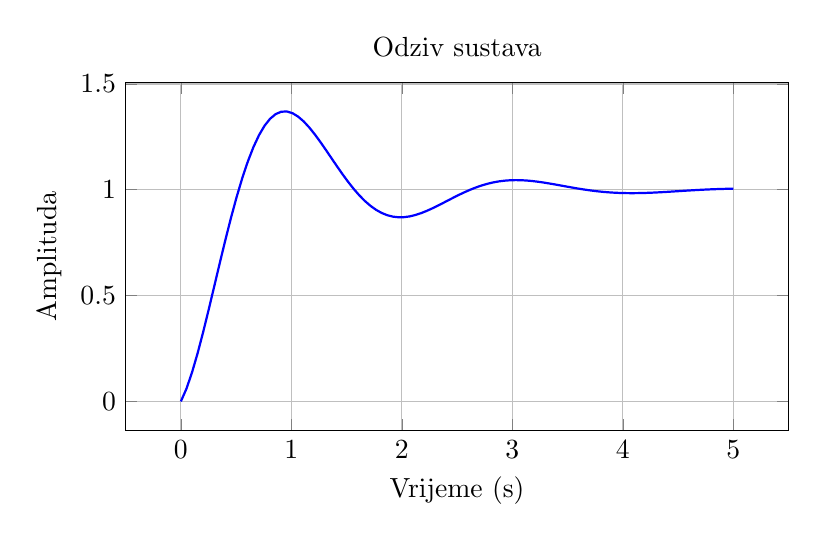
\begin{tikzpicture}
    \begin{axis}[
        width=10cm, height=6cm,
        xlabel={Vrijeme (s)},
        ylabel={Amplituda},
        grid=major,
        title={Odziv sustava}
    ]
    \addplot[blue, thick, domain=0:5, samples=100] {1 - exp(-x)*cos(deg(3*x))};
    \end{axis}
    \end{tikzpicture}
    \caption{Odziv simuliranog sustava na skokovitu pobudu}
    \label{fig:graf}
\end{figure}

\subsection{2.4. Optimizacija parametara}
Parametri su optimizirani korištenjem genetskog algoritma.

\section{3. ZAKLJUČAK}
Na temelju provedenih ispitivanja, može se zaključiti da predloženi sustav zadovoljava sve tehničke specifikacije i ostvaruje stabilno ponašanje u stvarnim uvjetima rada.

\end{document}
